\documentclass{article}
\usepackage[letterpaper, rmargin=3em, lmargin=3em, textheight=63em]{geometry}
\usepackage{fancyhdr}
\usepackage[spanish]{babel}
\usepackage[dvipsnames]{xcolor}
\usepackage{graphicx}
\usepackage{wrapfig}
\usepackage{setspace}
\usepackage{hyperref}

\usepackage{amssymb}
\usepackage{amsmath}

\usepackage{charter}
\usepackage{physics}

\usepackage{multicol}
\usepackage{tikz}
% GEOMETRY
\setlength{\parskip}{1em}
\pagestyle{fancy}
\lhead{Facultad de Ciencias Físicas y Matemáticas}
\rhead{Universidad de Chile}
\cfoot{ }

\renewcommand{\labelenumi}{\normalsize\bfseries P\arabic{enumi}.}
%\renewcommand{\labelenumii}{\normalsize\bfseries (\alph{enumii})}
\renewcommand{\labelenumiii}{\normalsize\bfseries \roman{enumiii})}

% Alfabeto
\newcommand{\A}{\mathcal{A}}
\newcommand{\B}{\mathcal{B}}
\newcommand{\C}{\mathcal{C}}
\newcommand{\E}{\mathcal{E}}
\newcommand{\F}{\mathcal{F}}
\newcommand{\I}{\mathcal{I}}
\newcommand{\K}{\mathcal{K}}
\renewcommand{\L}{\mathcal{L}}
\newcommand{\M}{\mathcal{M}}
\newcommand{\N}{\mathbb{N}}
\renewcommand{\P}{\mathcal{P}}
\newcommand{\Q}{\mathbb{Q}}
\newcommand{\R}{\mathbb{R}}
\renewcommand{\S}{\mathcal{S}}
\newcommand{\T}{\mathcal{T}}
\newcommand{\Z}{\mathbb{Z}}

\DeclareMathOperator{\sen}{sen}
\DeclareMathOperator{\senh}{senh}
\DeclareMathOperator{\tg}{tg}
\DeclareMathOperator{\dom}{dom}
\DeclareMathOperator{\dist}{dist}
\DeclareMathOperator*{\argmin}{argmin}
\DeclareMathOperator{\arccosh}{arccosh}

\renewcommand{\epsilon}{\varepsilon}
\renewcommand{\phi}{\varphi}
\newcommand{\dprod}[2]{\langle #1 , #2 \rangle}
\newcommand{\prox}{\mathbf{prox}}

\hypersetup{
    colorlinks=true,
    linkcolor=blue,
    filecolor=magenta,      
    urlcolor=blue,
}

\begin{document}
\noindent \textbf{MA3701 Optimización}\\
\textbf{Profesor:} Alejandro Jofré\\
\textbf{Auxiliar:} Benjamín Vera Vera


\begin{center}
    \Huge{\textbf{Auxiliar 3}}\\
\textit{\large{Condiciones de optimalidad}}\\
    \normalsize
    27 de agosto de 2025
\end{center}

\begin{enumerate}
	\item Considere el siguiente problema de optimización:
		\begin{align*}
			\min_{x \in \mathbb{R}^2} \; & x_1^2 + x_2^2 \\
						     & (x_1 - 1)^2 + (x_2 - 1)^2 \leq 1 \\
						     & (x_1 - 1)^2 + (x_2 + 1)^2 \leq 1.
		\end{align*}
		\begin{enumerate}
			\item Esboce el conjunto factible y los conjuntos de nivel de la función objetivo de este problema. Encuentre el minimizador \(x^*\).
			\item Obtenga las condiciones de KKT asociadas al problema. ¿Existen multiplicadores \(\lambda_1^*, \lambda_2^*\) asociados a \(x^*\)?
		\end{enumerate}
	\item Dado \(\alpha \geq 0\), considere el siguiente problema:
		\begin{align*}
			\min_{y_1, y_2} \; & y_1 \\
					   & y_1^2 - y_2 \leq \alpha, \\
					   & y_1^2 + y_2 \leq 0.
		\end{align*}
		Obtenga la solución de este problema y sus multiplicadores \(\lambda_1, \lambda_2 \geq 0\) asociados.

	\textit{Indicación:} Considere por separado los casos \(\alpha = 0, \alpha > 0.\)
\item Considere el sistema de resortes descrito en la figura \ref{fig:lal} en que los bloques tienen ancho \(w > 0\) y pueden chocar entre sí y con los muros.
\begin{figure}[h]
	\centering
	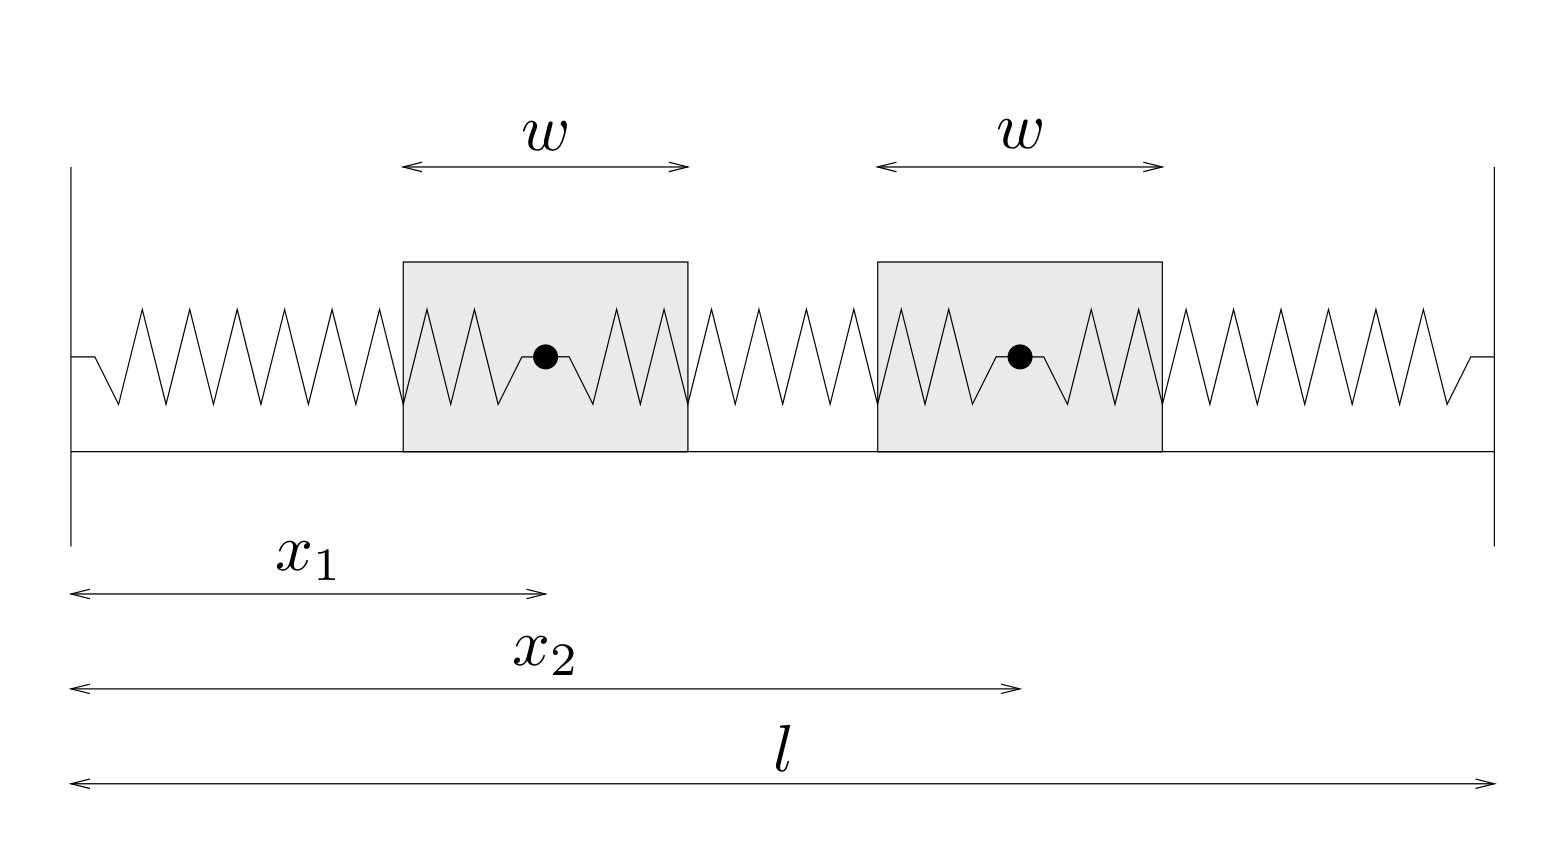
\includegraphics[width=0.7\textwidth]{img/spring.png}
	\caption{Sistema de resortes}
	\label{fig:lal}
\end{figure}
	\begin{enumerate}
		\item Plantee el problema de minimizar la energía potencial elástica del sistema dadas las fuerzas de contacto entre los bloques.
		\item Obtenga las condiciones de KKT de este problema y utilícelas para dar interpretación física a los multiplicadores de Lagrange en esta situación.
	\end{enumerate}
\end{enumerate}

\end{document}
